
%(BEGIN_QUESTION)
% Copyright 2006, Tony R. Kuphaldt, released under the Creative Commons Attribution License (v 1.0)
% This means you may do almost anything with this work of mine, so long as you give me proper credit

Conductance of an aqueous (water-based) solution is usually expressed in units of Siemens per centimeter (S/cm).  The unit of Siemens, of course, is nothing more than the reciprocal of Ohms, given that conductance ($G$) and resistance ($R$) are inverse quantities:

$$G = {1 \over R}$$

We may measure the conductivity of a liquid by immersing two electrodes of known area into that liquid, separating them by a known distance, and then measuring the electrical conductance between the electrodes.  We call such a device a {\it conductivity cell}:

$$\includegraphics[width=15.5cm]{i00606x01.eps}$$

Assuming the conductivity of the liquid does not change, how will the conductance measurement be affected by changes in electrode area and distance?  The following equation may be helpful in answering this question:

$$G = k{A \over d}$$

\noindent
Where,

$G$ = Conductance, in Siemens (S)

$k$ = Specific conductivity of liquid, in Siemens per centimeter (S/cm)

$A$ = Electrode area (each), in square centimeters (cm$^{2}$)

$d$ = Electrode separation distance, in centimeters (cm)

\vskip 10pt

Also, show how the unit of ``Siemens per centimeter'' comes directly from this equation.

\underbar{file i00606}
%(END_QUESTION)





%(BEGIN_ANSWER)

Here is a version of the conductivity cell equation showing units instead of variables:

$$[\hbox{S}] = \left[{\hbox{S} \over \hbox{cm}}\right]{[\hbox{cm}^2] \over [\hbox{cm}]}$$

\vskip 10pt

Follow-up question: identify the unit of conductance popular before Siemens.  Hint: it actually makes {\it sense} as opposed to being someone's (arbitrary) name!

%(END_ANSWER)





%(BEGIN_NOTES)

Conductance decreases with increasing area ($A$), and increases with increasing distance ($d$).

\vskip 10pt

The obsolete unit of conductance is the {\it mho}: ``ohm'' spelled backwards.  Cute, don't you think?  The symbol was even an upside-down Greek capital-letter omega!

%INDEX% Measurement, analytical: conductivity

%(END_NOTES)


